\section{Methodology}
\label{sec:method}

\begin{figure*}[t]
\centering
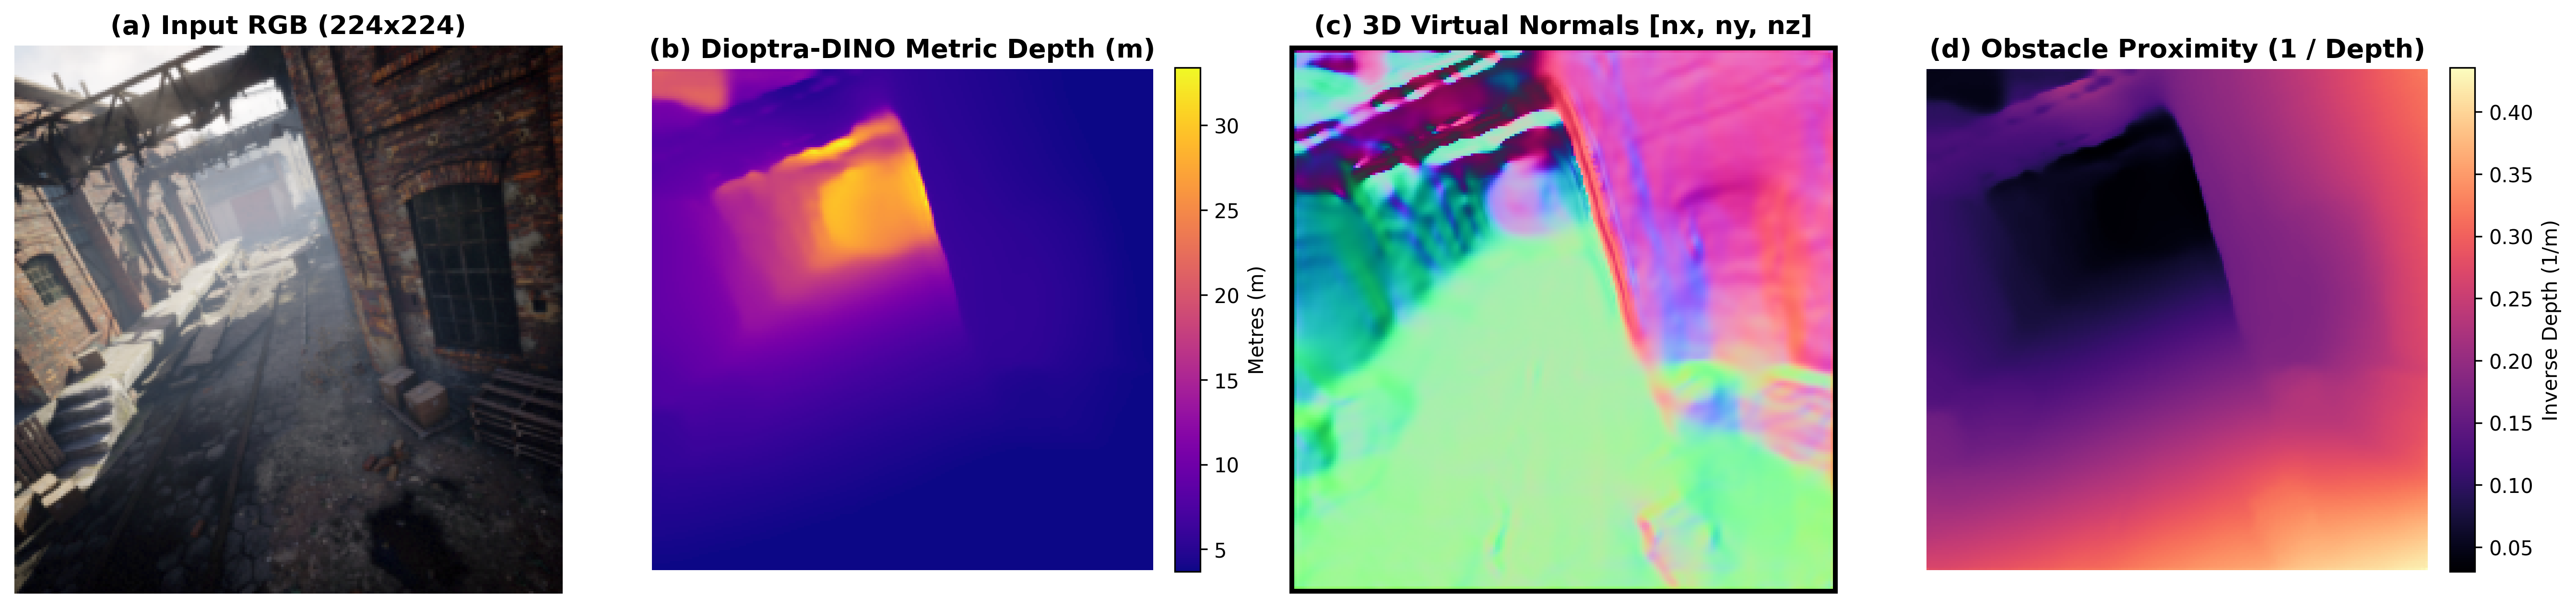
\includegraphics[width=\textwidth]{figures/fig_method_pipeline.png}
\caption{\textbf{Dioptra-DINO Architecture and Geometry-Coupled Training Framework}. An input RGB frame is processed by a self-supervised DINOv2-Small ViT backbone ($14 \times 14$ patches, $256$ tokens). Concurrently, camera intrinsics $\mathbf{K}'$ are unprojected into continuous 3D optical ray triplets $\mathcal{R}_i$, embedded via Fourier harmonics, and injected via affine FiLM modulation. Angular Residual Attention (ARA) introduces an intrinsic geometric penalty $\sin^2(\theta_{ij})$ into transformer self-attention. Multi-scale token features are reassembled via a DPT decoder supervised by a multi-task loss combining raw metric SiLog, batch log-median scale, edge gradients, and Multi-Scale 3D Virtual Normal Loss ($\mathcal{L}_{\text{vnl}}$). Dynamic pinhole crop augmentation enforces camera-intrinsic equivariance across continuous focal variations.}
\label{fig:pipeline}
\end{figure*}

\subsection{Architecture Overview}
Dioptra-DINO couples a self-supervised vision transformer backbone with physical projective camera constraints (Figure~\ref{fig:pipeline}). Given an RGB image $\mathbf{I} \in \mathbb{R}^{H \times W \times 3}$ and its camera intrinsic matrix $\mathbf{K} \in \mathbb{R}^{3 \times 3}$, our goal is to predict dense physical depth $\hat{\mathbf{D}} \in \mathbb{R}^{H \times W}$ in metres.

The network consists of:
\begin{enumerate}
    \item \textbf{Vision Backbone}: A pre-trained DINOv2-Small ViT (`vits14`, $21.66$\,M parameters) producing patch tokens $\mathbf{X}_0 \in \mathbb{R}^{N \times D}$, where $N = (H / 14) \times (W / 14) = 16 \times 16 = 256$ tokens and $D = 384$.
    \item \textbf{Trivision Ray Positional Encoding}: An analytic ray unprojection module that computes 3D optical unit rays and modulates patch tokens via affine Feature-wise Linear Modulation (FiLM).
    \item \textbf{Angular Residual Attention (ARA)}: A continuous geometric attention bias that penalizes divergent ray angles $\theta_{ij}$ across transformer attention heads.
    \item \textbf{Dense Prediction Transformer (DPT) Decoder}: A multi-scale reassembly and residual fusion decoder ($5.44$\,M parameters) generating full-resolution metric depth predictions.
\end{enumerate}

\subsection{Trivision Ray Positional Encoding}
Standard vision transformers rely on 2D coordinate embeddings that remain invariant under camera zoom or focal variations. To directly ground token representations in 3D projective space, we compute continuous optical unit rays for each patch.

Given a pixel $(u, v)$ and camera intrinsic calibration matrix $\mathbf{K}'$, the physical 3D optical ray direction is:
\begin{equation}
    \hat{\mathbf{r}}(u, v) = \frac{\mathbf{K}'^{-1} [u, v, 1]^T}{\|\mathbf{K}'^{-1} [u, v, 1]^T\|_2}
    \label{eq:ray_unproject}
\end{equation}

\noindent\textbf{Analytic Matrix Inversion}: To ensure numerical stability and avoid external linear algebra runtime dependencies on edge GPUs, we compute $\mathbf{K}'^{-1}$ in closed form via Cramer's rule:
\begin{equation}
    \mathbf{K}'^{-1} = \frac{\text{adj}(\mathbf{K}')}{\det(\mathbf{K}') + \epsilon}
\end{equation}
where $\det(\mathbf{K}') = f_x' f_y' > 0$ for standard cameras and $\epsilon = 10^{-8}$.

\noindent\textbf{Ray Triplet and Reflection Symmetry}: For each patch token centered at $(u_c, v_c)$ with half-width $p_h = P / 2$, we extract an optical ray triplet:
\begin{equation}
    \mathcal{R}_i = \left\{ \hat{\mathbf{r}}_{\text{center}}, \hat{\mathbf{r}}_{\text{corner1}}, \hat{\mathbf{r}}_{\text{corner2}} \right\}
\end{equation}
Under standard orientation, $\hat{\mathbf{r}}_{\text{corner1}}$ samples the top-left offset $(u_c - p_h, v_c - p_h)$ and $\hat{\mathbf{r}}_{\text{corner2}}$ samples the bottom-right offset $(u_c + p_h, v_c + p_h)$. When spatial data augmentation applies a horizontal reflection ($u' = W' - 1 - u$), we track this transformation and reflect the chiral corner rays:
\begin{equation}
    \hat{\mathbf{r}}_{\text{corner1}} \leftarrow (u_c + p_h, v_c - p_h), \quad \hat{\mathbf{r}}_{\text{corner2}} \leftarrow (u_c - p_h, v_c + p_h)
\end{equation}
This guarantees that optical ray directions correspond accurately to the augmented pixel contents.

\noindent\textbf{Multi-Frequency FiLM Modulation}: Each ray is embedded using multi-scale Fourier features across frequencies $k \in \{1, \dots, F\}$ with $F=6$:
\begin{equation}
    \gamma(\hat{\mathbf{r}}) = \left[ \sin(2^k \pi \hat{\mathbf{r}}), \cos(2^k \pi \hat{\mathbf{r}}) \right]_{k=1}^{F}
\end{equation}
The concatenated triplet embedding $\gamma(\mathcal{R}_i) \in \mathbb{R}^{108}$ is projected through a 2-layer MLP ($108 \rightarrow 256 \rightarrow 384$) with LayerNorm to generate affine scale $\alpha \in \mathbb{R}^{384}$ and shift $\beta \in \mathbb{R}^{384}$ vectors, modulating patch tokens via Feature-wise Linear Modulation: $\mathbf{x}' = \alpha \odot \mathbf{x} + \beta$.

\subsection{Angular Residual Attention (ARA)}
To refine high-frequency surface boundaries and encourage planar consistency, Dioptra introduces an intrinsic geometric attention bias. In a perspective optical frame, the angular separation $\theta_{q, k}$ between a query ray $\hat{\mathbf{r}}_q$ and key ray $\hat{\mathbf{r}}_k$ satisfies:
\begin{equation}
    d_{\text{ang}}^2(\hat{\mathbf{r}}_q, \hat{\mathbf{r}}_k) = 1 - (\hat{\mathbf{r}}_q \cdot \hat{\mathbf{r}}_k)^2 = \sin^2(\theta_{q, k})
\end{equation}

We define the Angular Residual Attention bias $\mathbf{B} \in \mathbb{R}^{H \times N \times N}$ for attention head $h$ as:
\begin{equation}
    \mathbf{B}_h(i, j) = -\frac{\alpha_h}{\sigma_h^2 + \epsilon} \sum_{m=1}^3 \sin^2(\theta(\hat{\mathbf{r}}_{i, m}, \hat{\mathbf{r}}_{j, \text{center}}))
    \label{eq:ara_bias}
\end{equation}
where $\alpha_h \in \mathbb{R}$ and $\sigma_h^2 \in \mathbb{R}$ are learnable per-head gain and bandwidth parameters initialized to $0.5$, and $m \in \{1, 2, 3\}$ sums over token $i$'s Trivision ray triplet against key token $j$'s principal center ray. 

Self-attention incorporating ARA is formulated as:
\begin{equation}
    \text{Attn}(\mathbf{Q}, \mathbf{K}, \mathbf{V}) = \text{Softmax}\left( \frac{\mathbf{Q}\mathbf{K}^T}{\sqrt{d_h}} + \Gamma(t) \cdot \mathbf{B} \right) \mathbf{V}
\end{equation}
where $\Gamma(t) \in [0, 1]$ is a smooth cosine warmup gate governed by epoch $t$:
\begin{equation}
    \Gamma(t) = \begin{cases} 
      0, & t < t_{\text{warmup}} \\
      \frac{1}{2}\left(1 - \cos\left(\pi \frac{t - t_{\text{warmup}}}{t_{\text{full}} - t_{\text{warmup}}}\right)\right), & t_{\text{warmup}} \le t \le t_{\text{full}} \\
      1, & t > t_{\text{full}}
   \end{cases}
\end{equation}
We set $t_{\text{warmup}} = 1$ and $t_{\text{full}} = 3$, allowing visual feature representations to stabilize before the geometric attention bias reaches full intensity.

\subsection{Decoupled Metric Scale \& Shape Supervision}
To prevent the model from collapsing into arbitrary scale-shifted predictions, we decouple global physical scale learning from local relative shape regularizers.

\noindent\textbf{1. Raw Metric SiLog Loss ($\mathcal{L}_{\text{SiLog}}$)}:
Unlike relative depth frameworks that normalize depth predictions per sample, our Scale-Invariant Logarithmic loss operates directly on unnormalized physical metric depths:
\begin{equation}
    \mathcal{L}_{\text{SiLog}} = \frac{1}{|V|} \sum_{i \in V} d_i^2 - \frac{\lambda}{|V|^2} \left( \sum_{i \in V} d_i \right)^2
\end{equation}
where $d_i = \log(\hat{\mathbf{D}}_i) - \log(\mathbf{D}_i^*)$, $\lambda = 0.85$, and $V$ denotes valid ground-truth pixels within the operational range $[0.1\,\text{m}, 80.0\,\text{m}]$.

\noindent\textbf{2. Global Scale Consistency Loss ($\mathcal{L}_{\text{scale}}$)}:
To explicitly supervise global metric scale, we compute the batch-averaged absolute log-median error:
\begin{equation}
    \mathcal{L}_{\text{scale}} = \frac{1}{B} \sum_{b=1}^B \left| \log(\text{median}(\hat{\mathbf{D}}_b)) - \log(\text{median}(\mathbf{D}_b^*)) \right|
\end{equation}
This directly penalizes overall physical scale drift across trajectories without interfering with local depth gradients.

\noindent\textbf{3. Multi-Scale 3D Virtual Normal Loss ($\mathcal{L}_{\text{vnl}}$)}:
To enforce planar architectural geometry and eliminate surface rippling, we introduce a Multi-Scale 3D Virtual Normal Loss inspired by~\cite{yin2019enforcing}. For predicted depth $\hat{\mathbf{D}}$ and ground truth $\mathbf{D}^*$, 3D point clouds in camera coordinate space are formed via backprojection:
\begin{equation}
    \mathbf{P}(u, v) = \left[ \frac{u - c_x}{f_x} \cdot D(u, v), \; \frac{v - c_y}{f_y} \cdot D(u, v), \; D(u, v) \right]^T
\end{equation}
For each spatial stencil dilation scale $s \in \mathcal{S} = \{1, 2, 4\}$, horizontal and vertical tangent vectors are formed:
\begin{equation}
\begin{aligned}
    \mathbf{v}_x^{(s)}(u, v) &= \mathbf{P}(u + s, v) - \mathbf{P}(u - s, v) \\
    \mathbf{v}_y^{(s)}(u, v) &= \mathbf{P}(u, v + s) - \mathbf{P}(u, v - s)
\end{aligned}
\end{equation}
The unnormalized surface normal is given by the spatial cross product:
\begin{equation}
    \mathbf{n}^{(s)}(u, v) = \mathbf{v}_x^{(s)}(u, v) \times \mathbf{v}_y^{(s)}(u, v)
\end{equation}
Unit normal vectors $\hat{\mathbf{n}}^{(s)} = \mathbf{n}^{(s)} / (\|\mathbf{n}^{(s)}\|_2 + \epsilon)$ are computed for both prediction ($\hat{\mathbf{n}}_{\text{pred}}^{(s)}$) and ground truth ($\hat{\mathbf{n}}_{\text{gt}}^{(s)}$). The virtual normal loss averages cosine angular deviation over valid inner pixels $\mathcal{M}^{(s)}$ across all dilation stencils:
\begin{equation}
    \mathcal{L}_{\text{vnl}} = \frac{1}{|\mathcal{S}|} \sum_{s \in \mathcal{S}} \frac{1}{|\mathcal{M}^{(s)}|} \sum_{(u, v) \in \mathcal{M}^{(s)}} \left( 1 - \hat{\mathbf{n}}_{\text{pred}}^{(s)}(u, v) \cdot \hat{\mathbf{n}}_{\text{gt}}^{(s)}(u, v) \right)
\end{equation}

\noindent\textbf{4. Multi-Scale Sobel Edge Loss ($\mathcal{L}_{\text{edge}}$)}:
To preserve sharp depth discontinuities across occlusion boundaries, horizontal and vertical Sobel filter responses are penalized against ground-truth gradients:
\begin{equation}
    \mathcal{L}_{\text{edge}} = \frac{1}{|V|} \sum_{i \in V} \left( \|\nabla_x \hat{\mathbf{D}}_i - \nabla_x \mathbf{D}_i^*\|_1 + \|\nabla_y \hat{\mathbf{D}}_i - \nabla_y \mathbf{D}_i^*\|_1 \right)
\end{equation}

\noindent\textbf{5. Multi-Task Objective}:
The complete optimization objective combines the four complementary terms:
\begin{equation}
    \mathcal{L}_{\text{total}} = w_{\text{silog}} \mathcal{L}_{\text{SiLog}} + w_{\text{scale}} \mathcal{L}_{\text{scale}} + w_{\text{edge}} \mathcal{L}_{\text{edge}} + w_{\text{vnl}} \mathcal{L}_{\text{vnl}}
\end{equation}
where loss balancing weights are set to $w_{\text{silog}} = 1.0, w_{\text{scale}} = 0.5, w_{\text{edge}} = 0.2$, and $w_{\text{vnl}} = 0.25$.

\subsection{Dynamic Pinhole Crop Augmentation}
\label{sec:dynamic_crop}
In datasets captured with a single virtual or physical camera, such as TartanAir~\cite{wang2020tartanair}, the camera intrinsic matrix $\mathbf{K}$ is static across all trajectories. Under this degenerate condition, the optical unprojection ray vector $\hat{\mathbf{r}}(u, v)$ in Eq.~\eqref{eq:ray_unproject} reduces to a deterministic function of 2D pixel coordinates $(u, v)$---mathematically indistinguishable from a learned spatial positional embedding. Under fixed-$\mathbf{K}$ training, the model can bypass physical camera conditioning, leaving it vulnerable to optical scale errors when deployed on sensors with different focal lengths or fields of view.

To enforce genuine camera-intrinsic equivariance, we introduce \textbf{Dynamic Pinhole Crop Augmentation}. During training, given an input frame with dimensions $W \times H$ and intrinsic matrix $\mathbf{K}$, we stochastically sample a square crop window of size $L$:
\begin{equation}
    L \sim \mathcal{U}(s_{\min} \cdot \min(W, H), \min(W, H)), \quad s_{\min} = 0.55
\end{equation}
with top-left corner $(x_0, y_0)$ sampled uniformly over the valid range $[0, W - L] \times [0, H - L]$. The cropped region is bilinearly resized to the network training resolution $W' \times H' = 224 \times 224$. 

Under projective pinhole geometry, spatial scaling and translation of the sensor plane transform the intrinsic parameters as:
\begin{equation}
\begin{aligned}
    f_x' &= f_x \cdot \frac{W'}{L}, \qquad &f_y' &= f_y \cdot \frac{H'}{L}, \\
    c_x' &= (c_x - x_0) \cdot \frac{W'}{L}, \qquad &c_y' &= (c_y - y_0) \cdot \frac{H'}{L}
\end{aligned}
\label{eq:pinhole_transform}
\end{equation}
Because the cropped region represents a magnified sub-cone of the optical frustum, the effective horizontal field of view varies continuously between $\approx 45.0^\circ$ and $73.7^\circ$ ($f \in [0.75f_0, 1.5f_0]$). Crucially, physical metric depth values $\mathbf{D}^*(u, v)$ in metres are invariant to sensor cropping. This transformation cleanly uncouples pixel positions $(u, v)$ from optical ray angles $\hat{\mathbf{r}}$, forcing the Trivision encoder and ARA attention bias to actively condition on the transformed intrinsic matrix $\mathbf{K}'$.

\subsection{Implementation and Training Details}
\label{sec:training_details}
Dioptra-DINO is implemented in PyTorch and trained on dual NVIDIA Tesla T4 GPUs ($32$\,GB total VRAM). We employ the AdamW optimizer with $\beta_1 = 0.9, \beta_2 = 0.999$, weight decay $\lambda = 0.05$, and decoupled learning rates: a base learning rate of $\eta_{\text{backbone}} = 2 \times 10^{-5}$ for the pretrained DINOv2-Small ViT backbone and $\eta_{\text{head}} = 2 \times 10^{-4}$ for newly initialized geometry and DPT decoder modules. Learning rates decay via a cosine annealing schedule over 26 epochs with a 2-epoch linear warmup. 

The batch size is set to 8 per GPU with gradient accumulation across 4 steps, yielding an effective batch size of 32. Mixed-precision arithmetic (FP16) via PyTorch AMP is enabled throughout training, with gradient norms clipped to $1.0$. Total training over 26 epochs ($18,464$ samples per epoch) required approximately $36$ GPU-hours.
